\documentclass[11pt]{article}

\usepackage{acl-hlt2011}
\usepackage{times}
\usepackage{latexsym}
\usepackage{amsmath}
\usepackage{multirow}
\usepackage{url}
\usepackage{graphicx}
\usepackage{subfig}

\setlength\titlebox{6.5cm}

\title{Joshua}

\author{Jonathan Weese${}^\dag$, Chris Callison-Burch${}^\dag$, \and Matt Post${}^\star$ \\
\textdagger\ Center for Language and Speech Processing \\
$\star$\ Human Language Technology Center of Excellence \\
Johns Hopkins University \\
Baltimore, MD}

\date{}

\begin{document}
\maketitle

\begin{abstract}
We present progress on Joshua, an open-source decoder for hierarchical
and syntax-based machine translation.  The main focus
is on describing Thrax, a flexible, open source synchronous
context-free grammar extractor using Apache Hadoop.  Thrax extracts
both hierarchical \cite{Chiang2007} and syntax-augmented machine
translation \cite{samt2006} grammars.  It is built on Apache Hadoop for efficient
distributed performance, and can easily be extended with
support for new grammars, feature functions, and output formats.  

In addition, we present a single parameterized script for running the
complete Joshua pipeline.  This script is built on top of CachePipe, a
simple wrapper around shell command invocations that uses SHA1 hashes
of explicitly-listed dependencies to avoid re-running commands when
unnecessary.
\end{abstract}

\section{Introduction}

Joshua is an open-sourced toolkit for hierarchical machine translation
of human languages.  The original version of Joshua was a
reimplementation of the Python-based Hiero machine-translation system
(cite), and it was later extended to support richer syntactic
formalisms, such as SAMT (cite).

This past year, development in Joshua has had a broad focus on
improving the experimental pipeline.  Machine translation makes
use of many different datasets, training procedures, and pre- and
post-processing techniques that can have large effects on translation
outcome and make direct comparisons between systems difficult.  In addition,
managing one's own experiments is also quite difficult, as there is no
widely-accepted systematic means of recording every last parameter
that might have affected an experiment.  To address these, the latest
version of Joshua includes the following projects:

\begin{enumerate}
\item \emph{Thrax}, an open-source parameterized grammar extractor
  capable of extracting both Hiero and SAMT grammars.  Thrax is highly
  configurable.
\item \emph{CachePipe}, an open-source project that implements a cached
  pipeline.  CachePipe is a simple wrapper that determines whether
  pipeline commands need to be re-run.  It does this by computing SHA1
  hashes of dependencies to determine whether any of them have changed.
\item \verb|pipeline.pl|.  In the spirit of Moses'
  \verb|train-factored-phrase-model.perl| and \verb|mert-moses.pl|, we
  provide a single script that implements the entire Joshua pipeline,
  from data preparation to test-set decoding and evaluation.
\end{enumerate}

\section{Thrax: grammar extraction}

In modern machine translation systems such as Joshua \cite{Joshua-WMT} and cdec \cite{cdec}, a translation model is often represented as a synchronous context-free grammar (SCFG). Formally, an SCFG may be considered as a tuple
$$(N,S,T_\sigma,T_\tau,G)$$
where $N$ is a set of nonterminal symbols of the grammar, $S \in N$ is the goal symbol, $T_\sigma$ and $T_\tau$ are the source- and target-side terminal symbol vocabularies, respectively, and $G$ is a set of {\em production rules} of the grammar.

Each rule in $G$ is of the form
$$X \to \langle \alpha , \gamma , \sim \rangle$$
where $X \in N$ is a nonterminal symbol, $\alpha$ is a (possibly mixed) sequence of symbols from $N \cup T_\sigma$, $\gamma$ is a (again, possibly mixed) sequence of symbols from $N \cup T_\tau$, and $\sim$ is a one-to-one correspondence between the nonterminal symbols of $\alpha$ and $\gamma$.

The language of an SCFG is a set of ordered pairs of strings. During decoding, the set of candidate translations of an input sentence $f$ is the set of all $e$ such that the pair $(f,e)$ is licensed by the translation model SCFG.

Each candidate $e$ is generated by applying a certain set of production rules $(r_1 \ldots r_n)$ in sequence. We may define the {\em cost} of applying each rule as
\begin{equation}
w(X \to \langle \alpha, \gamma \rangle) = \prod_i{\phi_i(X \to \langle \alpha , \gamma \rangle)^{\lambda_i}}
\end{equation}
where each $\phi_i$ is a {\em feature function} and $\lambda_i$ is the weight for $\phi_i$.
We define the total {\em translation model score} of candidate $e$ as
\begin{equation}
w_{TM}(e) = \prod_{i=1}^n{w(r_i)}
\end{equation}
In practice, this translation model score is combined with scores from other features, such as a language model, to produce an overall score for each candidate translation.

\subsection{Hiero and SAMT}

\begin{figure}[t]
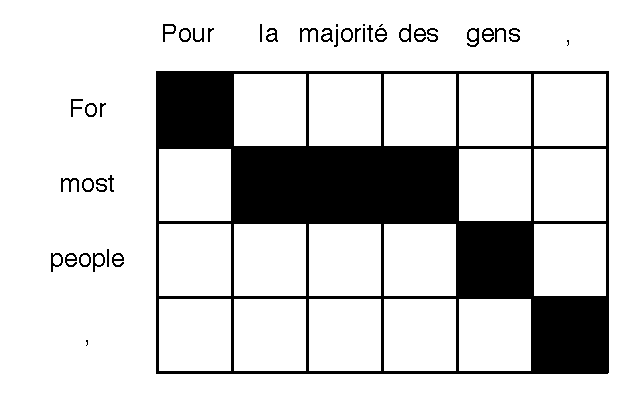
\includegraphics[width=0.5\textwidth]{figures/aligned-sentence}
\caption{A fragment of an aligned sentence pair.\label{aligned-sentence}}
\end{figure}

\begin{figure}[t]
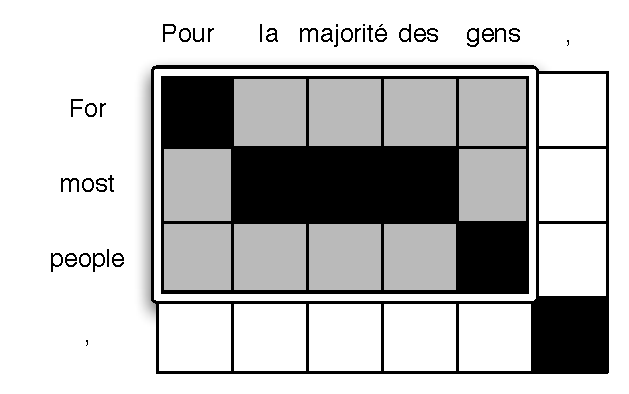
\includegraphics[width=0.5\textwidth]{figures/simple-rule}
\caption{A consistent phrase pair that can be extracted into the rule \\$X \to \langle \textrm{ Pour la majorit\'{e} des gens }; \textrm{ For most people } \rangle$.\label{hiero-rule}}
\end{figure}

\begin{figure}[t]
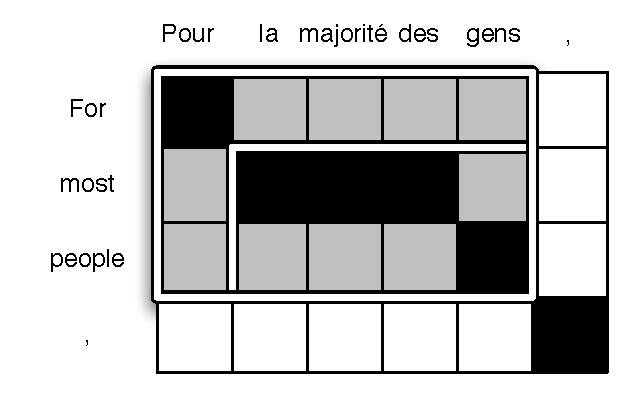
\includegraphics[width=0.5\textwidth]{figures/hierarchical-rule}
\caption{Two consistent phrase pairs that form the hierarchical rule $X \to \langle \textrm{ Pour } X ; \textrm{ For } X \rangle$.\label{hiero-rule-2}}
\end{figure}

Throughout this work, we will reference two particular SCFG types known as Hiero and Syntax-Augmented Machine Translation (SAMT).

A Hiero grammar \cite{Chiang2007} is an SCFG with only one type of nonterminal symbol (traditionally labelled $X$). A Hiero grammar can be extracted from a parallel corpus where each sentence pair has been word-aligned. An example of a sentence pair is shown in figure \ref{aligned-sentence}.

If $(f_i^j,e_k^l)$ is a sub-phrase of the sentence pair, we say it is {\em consistent} with the pair's alignment if none of the words in $f_i^j$ are aligned to words outside of $e_k^l$, and vice-versa. The consistent sub-phrase may be extracted as a SCFG rule as in figure \ref{hiero-rule}. Further, if a consistent phrase is contained within another one, a hierarchical rule may be extracted (see figure \ref{hiero-rule-2}).

An SAMT grammar \cite{samt2006} is similar to a Hiero grammar, except that the nonterminal symbols are syntactically motivated. SAMT rules are extracted from aligned sentence pairs, but they require some additional information: they require a parse tree for the target-side sentence.

When a rule is extracted as a consistent phrase pair (as in Hiero), if the target side is spanned by one constituent of the parse tree, we assign that constituent's label as the nonterminal symbol for the rule. Otherwise, we assign an extended category of the form $C_1+C_2$, $C_1 / C_2$, or $C_2$ \textbackslash $C_1$ --- indicating that the target side spans two adjacent constituents, is a $C_1$ missing a $C_2$ to the right, or is a $C_1$ missing a $C_2$ on the left, respectively. These extended categories are adapted from combinatory categorial grammars \cite{Steedman1999}.

\subsection{Related work}

We are not aware of any stand-alone grammar extraction programs. Other grammar extractors are developed and distributed with a particular MT system. We give an overview of a few such extractors here.

Joshua includes a simple Hiero extractor \cite{schwartz2010}. The extractor runs as a single Java process. This makes it difficult to extract larger grammars, as the host machine must have enough memory to hold all of the rules at once. Joshua's extractor scores each rule with three feature functions --- lexical probabilities in two directions, and one phrasal probability score $p(\gamma|\alpha)$. (These features are described in detail in section \ref{features}, since Thrax implements them as well.) 

The SAMT implementation of Zollmann and Venugopal \shortcite{samt2006} includes a several-thousand-line Perl script to extract their rules. In addition to phrasal and lexical probabilities, this extractor implements several other features that are also described in section \ref{features}.

Finally, the cdec decoder \cite {cdec} includes a rudimentary grammar extractor that performs well only when all rules can be held in memory.

Memory usage is a serious limitation of both Joshua and cdec extractors. Translation models can be very large, and many feature scores require accumulation of statistical data from the entire set of extracted rules. Since it is impractical to keep the entire grammar in memory, rules are usually sorted on disk and then read sequentially.

Different feature calculations may require different sort orders, leading to a linear workflow that alternates between sorting the grammar and calculating a feature score. To calculate more feature scores, more sorts have to be performed. This discourages the implementation of new features. For example, Joshua's built-in rule extractor calculates the phrasal probability $p(\gamma|\alpha)$ for each rule but, to save time, does not calculate its obvious counterpart $p(\alpha|\gamma)$, which would require another sort.

The SAMT extractor does not have a problem with large data sets. Indeed, SAMT has been extended \cite{venugopal2009hadoop} to run on Hadoop, an implementation of Google's MapReduce framework for efficient processing of large amounts of data. We will discuss Hadoop more in section \ref{design}.

None of these three extractors are designed for flexibility in terms of grammar extraction. The Joshua and cdec extractors only extract Hiero grammars, and Zollmann and Venugopal's extractor can only extract SAMT-style grammars. They are not designed to score arbitrary feature sets, either.

Since variation in translation models and feature sets can have a significant effect on translation performance, we have developed Thrax in order to make it easy to build and test new models. We hope it will encourage novel feature engineering.

\subsection{System overview}
\label{design}
\begin{figure*}
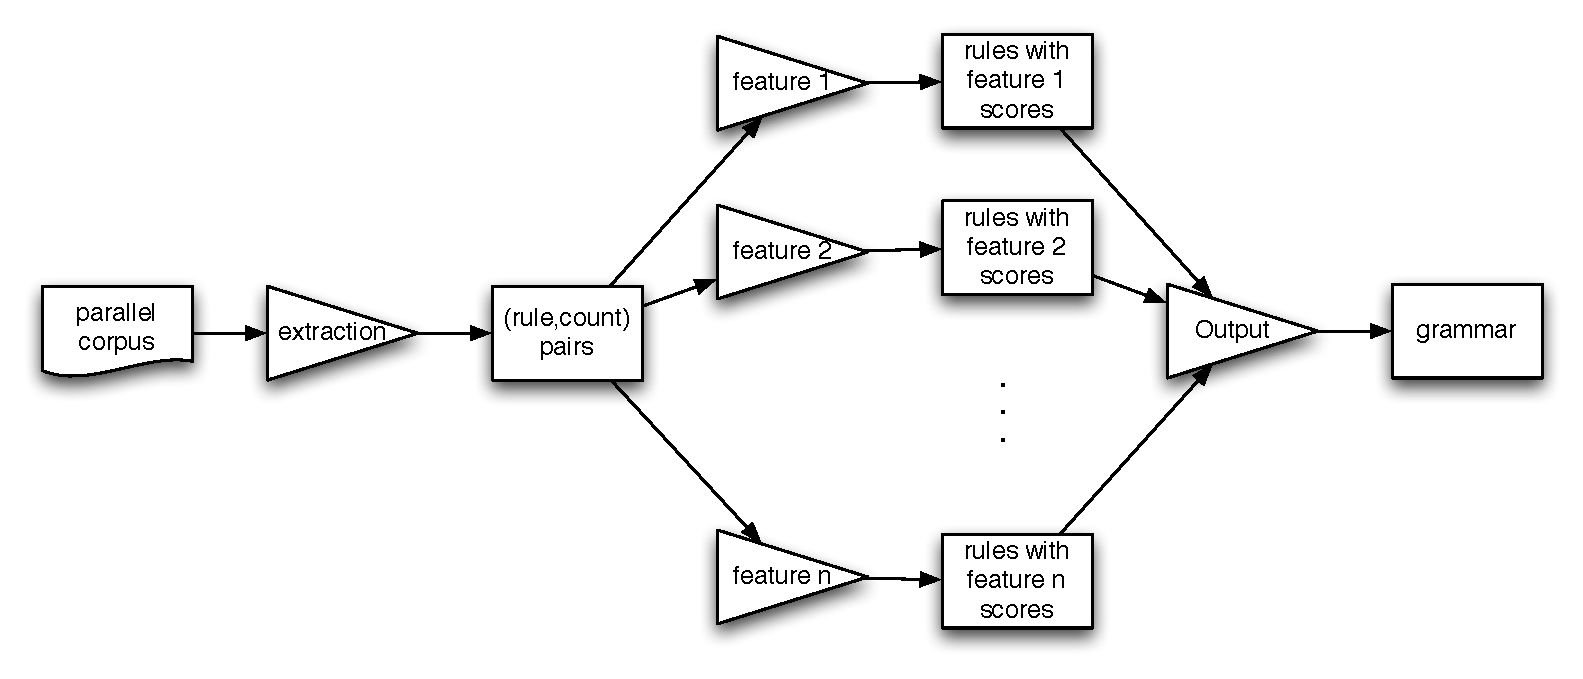
\includegraphics[width=6in]{figures/thrax-pipeline}
\caption{The Thrax pipeline. The right-pointing triangles are jobs that are submitted to a Hadoop cluster. Note that the feature jobs are all submitted in parallel.\label{thrax-workflow}}
\end{figure*}

To contrast with current grammar-extraction programs, we desire the following characteristics of Thrax:
\begin{itemize}
\item ability to extract different SCFGs (such as Hiero and SAMT), and to adjust various extraction parameters for the grammars;
\item ability to easily change the feature set with which to score the extracted rules, and easily implement new features;
\item scalability to arbitrarily large training corpora.
\end{itemize}

Thrax treats the grammar extraction and scoring as a series of dependent Hadoop jobs. Hadoop is an implementation of Google's MapReduce \cite{mapreduce}, a framework for distributed processing of large data sets. Hadoop jobs have two parts. In the {\em map} step, a set of key/value pairs is mapped to a set of intermediate key/value pairs. In the {\em reduce} step, all intermediate values associated with an intermediate key are merged.

The Thrax pipeline is shown in figure \ref{thrax-workflow}. The first step is to extract all the grammar rules. The map step in this job takes as input word-aligned sentence pairs and produces a set of ordered pairs $(r,c)$ where $r$ is a rule and $c$ is the number of times it was extracted. During the reduce step, these rule counts are summed, so the result is a set of rules, along with the total number of times each rule was extracted from the entire corpus.

Given the rules and their counts, a separate Hadoop job is run for each feature. These jobs can all be submitted at once and run in parallel, avoiding the linear sort-and-score workflow. The output from each feature job is the same set of pairs $(r,c)$ as the input, except each rule $r$ has been annotated with some feature score $f$.

After the feature jobs have been completed, we have several copies of the grammar, each of which has been scored with one feature. One last Hadoop job combines all these scores to produce the final grammar.

Some users may not have access to a Hadoop cluster. Thrax can be run in standalone or pseudo-distributed mode on a single machine. It can also be used with Amazon Elastic MapReduce\footnote{\url{http://aws.amazon.com/elasticmapreduce/}}, a web service that provides computation time on a Hadoop cluster on-demand.

\subsection{Extraction}

The first step in the Thrax workflow is the extraction of grammar rules from an input corpus. As mentioned above, Hiero and SAMT grammars both require a parallel corpus with word-level alignments. SAMT additionally requires that the target side of the corpus be parsed.

There are several parameters that can make a significant difference in a grammar's overall translation performance. Each of these parameters is easily adjustable in Thrax by changing its value in a configuration file.
\begin{itemize}
\item maximum rule span
\item maximum span of consistent phrase pairs
\item maximum number of nonterminals
\item minimum number of aligned terminals in rule
\item whether to allow adjacent nonterminals on source side
\item whether to allow unaligned words at the edges of consistent phrase pairs
\end{itemize}

Chiang \shortcite{Chiang2007} gives reasonable heuristic choices for these parameters when extracting a Hiero grammar, and Lopez \shortcite{lopez-2008} confirms some of them (maximum rule span, maximum number of source-side symbols, and maximum number of nonterminals). No similar parameter analysis has been performed for SAMT.

When extracting Hiero- or SAMT-style grammars, the first Hadoop job in the Thrax workflow takes in a parallel corpus and produces a set of rules. But in fact Thrax's extraction mechanism is more general than that; all it requires is a function that maps a string to a set of rules. This makes it easy to implement new grammars and extract them using Thrax.

\subsection{Feature functions}
\label{features}

Thrax considers feature functions of two types: first, there are features that can be calculated by looking at each rule in isolation. Such features do not require a Hadoop job to calculate their scores, since we may inspect the rules in any order. (In practice, we calculate the scores at the very last moment before outputting the final grammar.) We call these features {\em simple features}. Thrax implements the following simple features:
\begin{itemize}
\item a binary indicator function if the rule is purely abstract (with no terminal symbols);
\item an indicator function if the rule is purely lexical (with no nonterminals);
\item an indicator function if the rule is monotonic or has reordering;
\item an indicator function if the rule has adjacent nonterminals on the source side;
\item a counter giving the number of unaligned words in the rule;
\item a counter giving the number of terminals on the target side of the rule;
\item a constant phrase penalty.
\end{itemize}
In addition to simple features, Thrax also implements {\em map-reduce features}. These are features that require a Hadoop job to calculate, because the rules must be compared to each other in a certain order. Thrax implements the following map-reduce features:
\begin{itemize}
\item Phrasal translation probabilities $p(\alpha|\gamma)$ and $p(\gamma|\alpha)$. These are calculated by relative frequency:
\begin{equation}
p(\alpha|\gamma) = \frac{C(\alpha,\gamma)}{C(\gamma)}
\end{equation}
\begin{equation}
p(\gamma|\alpha) = \frac{C(\alpha,\gamma)}{C(\alpha)}
\end{equation}
where $C(\cdot)$ is the number of times a rule with the given source or target (or both) was extracted.
\item Lexical weighting $p_{\textit{lex}}(\alpha|\gamma,A)$ and $p_{\textit{lex}}(\gamma|\alpha,A)$. We calculate these weights as given in \cite{koehn2003}: let $A$ be the alignment between $\alpha$ and $\gamma$, so $(i,j) \in A$ if and only if the $i$th word of $\alpha$ is aligned to the $j$th word of $\gamma$. Then we can define $p_{\textit{lex}}(\gamma|\alpha)$ as
\begin{equation}
\prod_{i=1}^n{\frac{1}{|\{j : (i,j) \in A\}|}\sum_{(i,j) \in A}{w(\gamma_j|\alpha_i)}}
\end{equation}
where $\alpha_i$ is the $i$th word of $\alpha$, $\gamma_j$ is the $j$th word of $\gamma$, and $w(y|x)$ is the probability of seeing word $y$ given $x$, estimated by relative frequency.
\item Rarity penalty, given by
\begin{equation}
\exp(1 - C(X \to \langle \alpha , \gamma \rangle))
\end{equation}
where again $C(\cdot)$ is a count of the number of times the rule was extracted over the entire corpus.
\end{itemize}

Each of the features we mentioned above can be individually included or excluded when the grammar is extracted. One can simply list the features to be included in a configuration file.

It is very easy to extend Thrax with new feature functions. For simple features, all that is needed is a method that takes in a rule and calculates a feature score. Map-reduce features are slightly more complex: one must define a mapper and reducer, but also a sort comparator to determine in what order the rules are compared during the reduce step.


\section{The Joshua pipeline}

Machine translation systems require the specification and execution of
many steps, including:

\begin{enumerate}
\item Tokenizing, shortening, and recasing the training, tuning, and test data
\item Aligning the training corpora
\item Optionally parsing one or both sides of the input
\item Extracting phrase tables and hierarchical grammars
\item Tuning the parameters of the model
\item Optionally detokenizing and recasing
\item Evaluation
\end{enumerate}

\noindent Each of these high-level steps is controlled by any number
of parameters and broken down further into sub-steps, leading to
significant complication in maintaining, repeating, and comparing
experimental results.

Building and managing pipelines --- both as a record of what was done,
and a means of reproducing it in the future --- is often left to individual
researchers.  This is a problem especially for publicly available open-source
toolkits, like Joshua, that are improved and extended, or used as
black-box baselines.

The Moses decoder provides scripts that automate the pipeline
(e.g., \verb|train-factored-phrase-model.perl| and \verb|mert-moses.pl|).
In this spirit, we have written a single script that runs the entire
Joshua pipeline, effectively implementing the detailed step-by-step
instructions already available
online.\footnote{\url{http://www.cs.jhu.edu/~ccb/joshua/index.html}}
The script, distributed with the Joshua source code, minimally
requires the source and target language extensions and path prefixes
for training, tuning, and development data.  It follows many of the
command-line conventions of the Moses scripts.  It has the following
non-exhaustive feature set:

\begin{itemize}
\item run only a piece of the pipeline by specifying pre-defined start
  and stop steps
\item optionally subsample the corpus towards the development data
\item extract and decode with either Hiero or SAMT grammars
\item skip steps by providing the information produced by that
  step
\item recase and detokenize
\item evaluate
\end{itemize}

\noindent The script is written in Perl and is well-documented.

\section{CachePipe: Cached pipeline runs}

Some commands in the MT pipeline are very expensive to run, taking
hours or even days to complete.  There are many situations in which a
command does not need to be re-run, and it would be nice to have a
system which could make those determinations.  Exactly how such a
determination is made is not always obvious or easy to specify, and
many systems have been proposed to help manage this problem, such as
Experiment.perl,\footnote{\url{http://www.statmt.org/moses/?n=FactoredTraining.EMS}},
LoonyBin \cite{clark2010loonybin}.

These systems all vary in how they make the caching determination, in
complexity and extensibility, and in ease of use.  

Our solution to the caching dependency problem is CachePipe.
CachePipe is designed with the following goals:

\begin{enumerate}
\item Ease of use, requiring minimal editing of existing scripts
\item Robust content-based dependency system
\end{enumerate}

\noindent CachePipe is essentially a wrapper for shell commands that
only runs the command if necessary.  Presented with a command to run
and a list of file dependencies, it works by computing SHA1 hashes of
the dependencies and of the command invocation and storing them; it
then executes the command only if any of those hashes are different
from previous runs.  

CachePipe is implemented as a Perl module, for easy incorporation into
existing Perl scripts.  It also works in shell scripts.  A basic
invocation involves the following components:

\begin{itemize}
\item a name or identifier associated with the command or step
\item the command to run
\item a list of file dependencies
\end{itemize}

\noindent For example, to copy file \verb|a| to \verb|b|, the
following shell command could be used:

\verb|cachecmd copy "cp a b" a b|

\noindent The use of SHA1 hashes results in a much more robust system than
timestamp-based determinations, especially in networked environments
where timestamps may differ slightly across machines.

Since it is built on CachePipe, the Joshua's pipeline command can be
safely re-run from start to finish.

\section{Future work}

As of this writing, Thrax is limited to SCFG-based translation models.
A natural development would be to extract GHKM grammars
\cite{galley2004what} or more recent tree-to-tree models
\cite{zhang2008,liu2009,chiang2010}.  We also hope that Thrax will
continue to be extended with more feature functions as researchers
develop and contribute them.

%% \section{Acknowledgments}
%% - grants
%% - Adam Lopez for help brainstorming CachePipe

\bibliographystyle{acl}
\bibliography{thrax}

\end{document}
